\begin{wrapfigure}[27]{r}{0.44\textwidth}
	\vspace{-\normalbaselineskip}
	\centering
	\begin{subfigure}[b]{0.4\textwidth}
		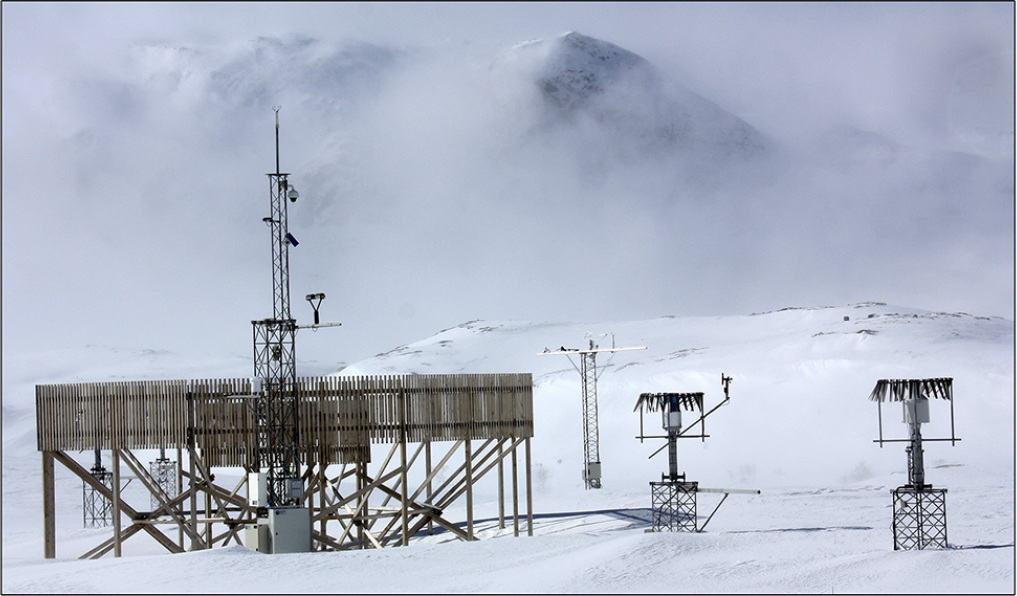
\includegraphics[width=\textwidth]{./fig_instruments/Dofe.png}
		\caption{}\label{fig:dofe_pic}
	\end{subfigure}	
	\begin{subfigure}[b]{0.4\textwidth}
		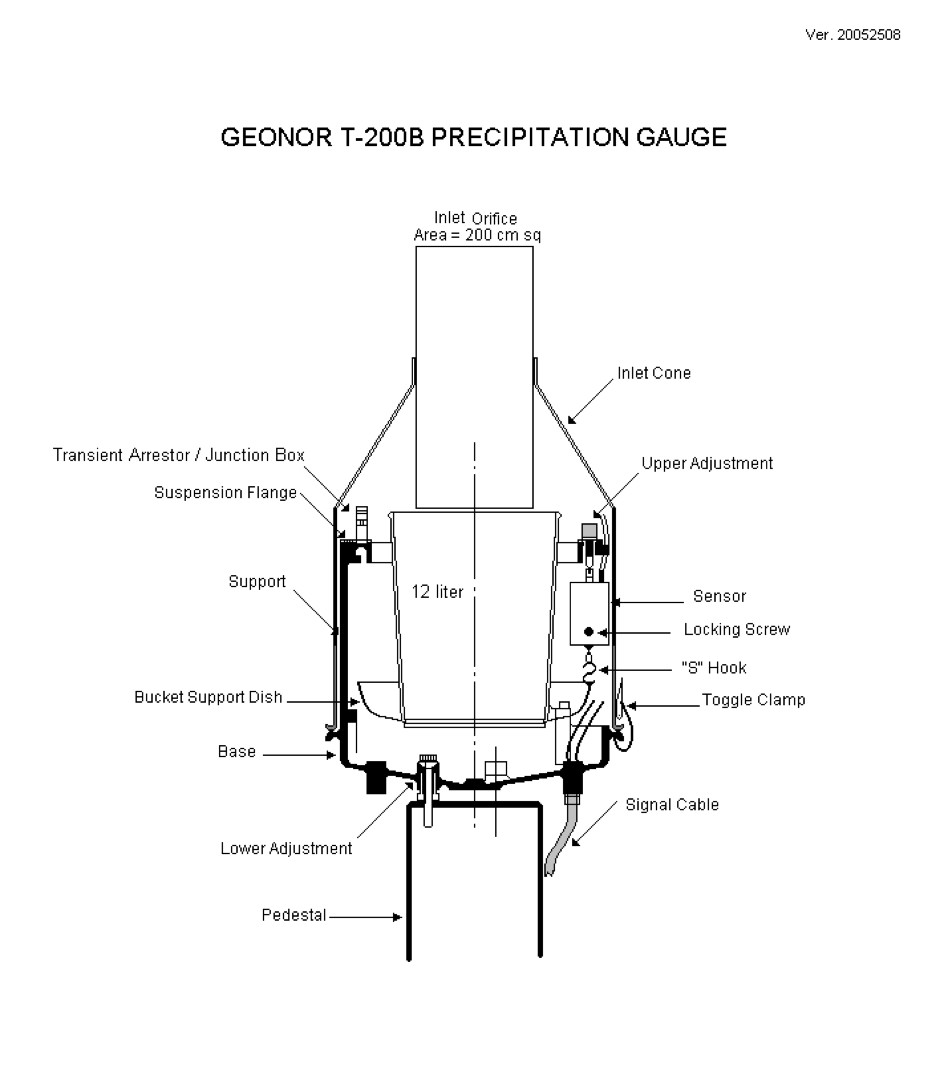
\includegraphics[trim={0.8cm, 2.3cm, 2.4cm, 3cm},clip,width=\textwidth]{./fig_instruments/Geonor_sketch.png}
		\caption{}\label{fig:gauge_sketch}
	\end{subfigure}	
	\caption{\protect\subref{fig:dofe_pic}: Double fence and unprotected precipitation gauges at Haukeliseter, from \cite{wolff_derivation_2015}. The prevailing wind direction from east comes from the lower, left corner in the image and the west wind from the opposite site. \protect\subref{fig:gauge_sketch}: Vertical cross section of T-200B precipitation gauge \citep{geonor_inc._t-200b_2015}.}\label{fig:Dofe}
	%	\vspace{-\normalbaselineskip}
\end{wrapfigure}